\documentclass[12pt]{article}

\usepackage{graphicx}
\usepackage{url}
\usepackage[utf8]{inputenc}
\usepackage{amsmath} % Para fórmulas matemáticas
\usepackage{amssymb} % Para símbolos matemáticos
\usepackage{geometry} % Para ajustar as margens
\usepackage{ragged2e} % Para \justifying
\usepackage{multirow}
\usepackage{hyperref} % Links
\usepackage{times}
\usepackage{tabularx}

\usepackage{xcolor}
\newcommand\todoe[1]{\textcolor{red}{evandro:#1}}

\usepackage{tocloft}      
\renewcommand{\cftsecleader}{\cftdotfill{\cftdotsep}}
\renewcommand{\cftdotsep}{.5}
\setlength{\cftbeforesubsecskip}{\cftbeforesecskip}
\renewcommand{\cftsubsecfont}{\cftsecfont}
\renewcommand{\cftsubsecpagefont}{\cftsecpagefont}
\setlength{\cftpartindent}{0em}
\setlength{\cftsecindent}{0em}
\setlength{\cftsubsecindent}{0em}
\setlength{\cftsubsubsecindent}{0em}

% Definição das margens (conforme especificado no template SBC)
\geometry{
  top=3.0cm,
  bottom=2.0cm,
  left=3.0cm,
  right=2.0cm
}

\usepackage{fancyhdr} % Para remover cabeçalho e rodapé
\pagestyle{empty} % Remove cabeçalho e rodapé de todas as páginas

\sloppy % Evita quebras de linha muito feias

% ===================================================================
% INFORMAÇÕES CENTRALIZADAS DO TRABALHO
% ===================================================================

% --- Autor ---
\newcommand{\autor}{Gabriella Marreto Rodrigues}
\newcommand{\citacaoAutor}{MARRETO, Gabriella} 
\newcommand{\mail}{gabriella.21@alunos.utfpr.edu.br}

% --- Título ---
\newcommand{\titulo}{Uma Arquitetura Cache-First para Aplicações PWA de Agendamento em Larga Escala Focada no Microempreendedor}
\newcommand{\tituloUppercase}{\MakeUppercase{\titulo}}
\newcommand{\titulotraduzido}{A Cache-First Architecture for Large-Scale PWA Scheduling Applications Focused on the Micro-entrepreneur}

% --- Resumo e Abstract ---
\newcommand{\textoResumo}{O microempreendedor brasileiro enfrenta desafios diários na gestão de agendamentos, recorrendo a métodos ineficientes como WhatsApp. Soluções de mercado existentes são complexas e caras (ex: Booksy) ou modelos \textit{freemium} limitados (ex: Reservio), além de não serem otimizadas para a realidade da conectividade precária de algumas regiões do país. Este trabalho propõe uma arquitetura \textit{Cache-First}, utilizando Supabase (Postgres, Auth com RLS, Edge Functions), Upstash (Redis) e Resend (Email). Essa solução garante alta performance e baixo consumo de dados. A arquitetura demonstra ser escalável, segura através de transações ACID e RLS, e economicamente viável, entregando uma experiência de usuário rápida e profissionalizando o serviço do de Microempreendedores com um baixo custo operacional.}

\newcommand{\textoAbstract}{azilian micro-entrepreneurs face daily challenges in managing appointments, often relying on inefficient methods such as WhatsApp. Existing market solutions are either complex and expensive (e.g., Booksy) or rely on limited \textit{freemium} models (e.g., Reservio), and they are not optimized for the reality of poor connectivity in some regions of the country. This work proposes a Cache-First architecture using Supabase (Postgres, Auth with RLS, Edge Functions), Upstash (Redis), and Resend (Email). This solution ensures high performance and low data consumption. The architecture proves to be scalable, secure through ACID transactions and RLS, and economically viable, delivering a fast user experience and professionalizing the service of micro-entrepreneurs with low operational costs.}

% --- Outras Informações ---
\newcommand{\orientador}{Prof. Dr. Nome do Orientador}
\newcommand{\datadeaprovacao}{Dia de Mês de 2025}
\newcommand{\instituicao}{UNIVERSIDADE TECNOLÓGICA FEDERAL DO PARANÁ}
\newcommand{\ano}{\the\year{}}

% --- Membros da Banca ---
\newcommand{\membroUm}{Prof. Dr. Nome do Membro 1}
\newcommand{\titulacaoMembroUm}{Doutorado}
\newcommand{\instituicaoMembroUm}{Instituição do Membro 1}
\newcommand{\membroDois}{Prof. Dr. Nome do Membro 2}
\newcommand{\titulacaoMembroDois}{Doutorado}
\newcommand{\instituicaoMembroDois}{Instituição do Membro 2}
\newcommand{\membroTres}{Prof. Dr. Nome do Membro 3}
\newcommand{\titulacaoMembroTres}{Doutorado}
\newcommand{\instituicaoMembroTres}{Instituição do Membro 3}

% ===================================================================
% CONFIGURAÇÃO DO CABEÇALHO DO ARTIGO (SBC TEMPLATE)
% Estas informações agora utilizam os comandos definidos acima.
% ===================================================================

% AJUSTE 1: O comando \title agora usa a variável \titulo.
\title{\titulo}

% AJUSTE 2: O comando \author agora usa a variável \autor.
\author{\autor}

\renewcommand{\contentsname}{SUMÁRIO}

\providecommand{\UTFPRlicencadata}{}
\newcommand{\licenca}[1]{\renewcommand{\UTFPRlicencadata}{#1}}

\newcommand{\licencaBy}{
    \begin{tabular}{cp{12.3cm}}
    	            \multirow{3}{*}{
\includegraphics[width=2.7cm]{licenses/by.png}}
    	            &
    	            {\fontsize{9}{9}\selectfont \parbox[t]{12.3cm}{Esta licença permite compartilhamento, remixe, adaptação e criação a partir do trabalho, mesmo para fins comerciais, desde que sejam atribuídos créditos ao(s) autor(es). Conteúdos elaborados por terceiros, citados e referenciados nesta obra não são cobertos pela licença.}} \\
    	            {\fontsize{9}{9}\selectfont\href{https://creativecommons.org/licenses/by/4.0/deed.pt_BR}{4.0 Internacional}} &
    	        \end{tabular}
                }

\newcommand{\licencaByNc}{
    \begin{tabular}{cp{12.3cm}}
    	            \multirow{3}{*}{
\includegraphics[width=2.7cm]{licenses/by-nc.png}}
    	            &
    	            {\fontsize{9}{9}\selectfont \parbox[t]{12.3cm}{Esta licença permite remixe, adaptação e criação a partir do trabalho, para fins não comerciais, desde que sejam atribuídos créditos ao(s) autor(es). Conteúdos elaborados por terceiros, citados e referenciados nesta obra não são cobertos pela licença.}} \\
    	            {\fontsize{9}{9}\selectfont\href{https://creativecommons.org/licenses/by-nc/4.0/deed.pt_BR}{4.0 Internacional}} &
    	        \end{tabular}}


\newcommand{\licencaByNcNd}{
    \begin{tabular}{cp{12.3cm}}
    	            \multirow{3}{*}{
\includegraphics[width=2.7cm]{licenses/by-nc-nd.png}}
    	            &
    	            {\fontsize{9}{9}\selectfont \parbox[t]{12.3cm}{Esta licença permite download e compartilhamento do trabalho desde que sejam atribuídos créditos ao(s) autor(es), sem a possibilidade de alterá-lo ou utilizá-lo para fins comerciais. Conteúdos elaborados por terceiros, citados e referenciados nesta obra não são cobertos pela licença.}} \\
    	            {\fontsize{9}{9}\selectfont\href{https://creativecommons.org/licenses/by-nc-nd/4.0/deed.pt_BR}{4.0 Internacional}} &
    	        \end{tabular}}


\newcommand{\licencaByNcSa}{
    \begin{tabular}{cp{12.3cm}}
    	            \multirow{3}{*}{
\includegraphics[width=2.7cm]{licenses/by-nc-sa.png}}
    	            &
    	            {\fontsize{9}{9}\selectfont \parbox[t]{12.3cm}{Esta licença permite remixe, adaptação e criação a partir do trabalho, para fins não comerciais, desde que sejam atribuídos créditos ao(s) autor(es) e que licenciem as novas criações sob termos idênticos. Conteúdos elaborados por terceiros, citados e referenciados nesta obra não são cobertos pela licença.}} \\
    	            {\fontsize{9}{9}\selectfont\href{https://creativecommons.org/licenses/by-nc-sa/4.0/deed.pt_BR}{4.0 Internacional}} &
    	        \end{tabular}}


\newcommand{\licencaByNd}{
    \begin{tabular}{cp{12.3cm}}
    	            \multirow{3}{*}{
\includegraphics[width=2.7cm]{licenses/by-nd.png}}
    	            &
    	            {\fontsize{9}{9}\selectfont \parbox[t]{12.3cm}{Esta licença permite compartilhamento do trabalho, mesmo para fins comerciais, sem a possibilidade de alterá-lo, desde que sejam atribuídos créditos ao(s) autor(es). Conteúdos elaborados por terceiros, citados e referenciados nesta obra não são cobertos pela licença.}} \\
    	            {\fontsize{9}{9}\selectfont\href{https://creativecommons.org/licenses/by-nd/4.0/deed.pt_BR}{4.0 Internacional}} &
    	        \end{tabular}}


\newcommand{\licencaBySa}{
    \begin{tabular}{cp{12.3cm}}
    	            \multirow{3}{*}{
\includegraphics[width=2.7cm]{licenses/by-sa.png}}
    	            &
    	            {\fontsize{9}{9}\selectfont \parbox[t]{12.3cm}{Esta licença permite remixe, adaptação e criação a partir do trabalho, mesmo para fins comerciais, desde que sejam atribuídos créditos ao(s) autor(es) e que licenciem as novas criações sob termos idênticos. Conteúdos elaborados por terceiros, citados e referenciados nesta obra não são cobertos pela licença.}} \\
    	            {\fontsize{9}{9}\selectfont\href{https://creativecommons.org/licenses/by-sa/4.0/deed.pt_BR}{4.0 Internacional}} &
    	        \end{tabular}}


\begin{document}

% Capa
\begin{titlepage}
\centering
{\large \instituicao} \\
\vspace*{4cm}
{\large \autor \par}
\vspace{6cm}
{\large \tituloUppercase \par}
\vspace*{\fill}
{\large DOIS VIZINHOS \par}
{\large \ano \par}
\end{titlepage}

\newpage
\pagestyle{empty}

% Folha de Rosto
\begin{titlepage}
\centering
{\large \autor \par}
\vspace{6cm}
{\large \tituloUppercase \par}
\vspace{1cm}
{\large \textbf{\titulotraduzido} \par}
\vspace{4cm}

\hfill
\parbox[t]{8cm}{

{Trabalho de Conclusão de Curso de Graduação apresentado como requisito parcial para a obtenção do título de Bacharel em Engenharia de Software, Universidade Tecnológica Federal do Paraná (UTFPR). \par}
\vspace{0.5cm}
{Orientador(a): Prof. Dr. Evandro Kuszera \par}
}

\vspace*{\fill}

{\large DOIS VIZINHOS \par}
{\large \ano \par} 

{
\licencaBySa 
}

\vspace{-1.5cm}

\end{titlepage}

\newpage
\pagestyle{empty}

% Folha de Aprovação
\begin{titlepage}
\centering
{\large \autor \par}
\vspace{1.5cm}
{\large \tituloUppercase \par}
\vspace{2cm}
\hfill
\parbox[t]{8cm}{
{Trabalho de Conclusão de Curso de Graduação apresentado como requisito para obtenção do título de Bacharel em Engenharia de Software, Universidade Tecnológica Federal do Paraná (UTFPR). \par}
}

\vspace{1.5cm}

{Data de aprovação: \datadeaprovacao \par}
\vspace{1.5cm}
\hrulefill 
%\vspace{-0.3cm}

{\membroUm}\\
{\titulacaoMembroUm}\\
{\instituicaoMembroUm}
\vspace{1cm}

\hrulefill 
%\vspace{-0.3cm}

{\membroDois} \\
{\titulacaoMembroDois} \\
{\instituicaoMembroDois} \\
\vspace{1cm}

\hrulefill 
%\vspace{-0.3cm}

{ \membroTres} \\
{ \titulacaoMembroTres} \\
{ \instituicaoMembroTres} \\

\vspace*{\fill}
{\large DOIS VIZINHOS \par}
{\large \ano \par}
\end{titlepage}

\newpage
\pagestyle{empty}

% Resumo
\centering
{ \textbf{RESUMO} \par}
\vspace{1cm}
\justifying

\noindent
\textoResumo

\vspace{1cm}
\noindent
Palavras-chave: Agendamento Online; PWA; Arquitetura Cache-First; Supabase; Microempreendedor (MEI).

\newpage
\pagestyle{empty}

% Abstract
\centering
{ \textbf{ABSTRACT} \par}
\vspace{1cm}
\justifying

\noindent
\textoAbstract

\vspace{1cm}
\noindent
Keywords: Online Scheduling; PWA; Cache-First Architecture; Supabase; Micro-entrepreneur (MEI).

\newpage
\pagestyle{empty}

% SUMÁRIO
\centering
{ \textbf{SUMÁRIO} \par}
\vspace{1cm}
\justifying

\renewcommand{\contentsname}{}
\pdfbookmark[0]{\contentsname}{toc}
\tableofcontents
\maketitle

\newpage
\pagestyle{plain} 
\pagenumbering{arabic}

%====================================================================

\section{Introdução}
\label{sec:introducao}

O Brasil vive um cenário econômico onde mais de 14,6 milhões de Microempreendedores Individuais (MEIs) \cite{ibge_noticias} sustentam a base da pirâmide de serviços. Para esse contingente massivo, a gestão do tempo não é apenas uma tarefa administrativa, mas um gargalo operacional. A realidade, no entanto, é arcaica: a dependência de métodos manuais, como agendas de papel, ou a troca trabalhosa de mensagens via WhatsApp, resulta em ineficiência crônica, erros humanos como choque de horários e perda direta de faturamento \cite{gov_mapa_empresas}.

Apesar da vasta oferta de ferramentas digitais, existe uma lacuna no mercado. As soluções de agendamento atuais falham em atender o MEI brasileiro, dividindo-se em categorias que ignoram a realidade financeira ou técnica desse público \cite{sebrae_digital}:

\begin{itemize}
    \item \textbf{Sistemas Enterprise/Complexos:} Plataformas como Booksy\footnote{https://booksy.com/pt-br/} e Trinks\footnote{https://negocios.trinks.com/planos/} são projetadas para PMEs (salões e clínicas com múltiplos funcionários), focando em gestão de estoque e comissões. O custo de assinatura (frequentemente acima de R\$ 99,00/mês) torna-se proibitivo para o profissional autônomo.
    \item \textbf{Modelos "Isca" (Freemium):} Ferramentas como Reservio\footnote{https://www.reservio.com/pt-br} e Minha Agenda Virtual atraem pelo "gratuito", mas impõem limitações severas (como teto de agendamentos mensais) que inviabilizam a operação real, servindo apenas como barreiras artificiais para forçar um \textit{upgrade}.
    \item \textbf{Softwares "Data-Heavy":} A grande maioria das aplicações web atuais (ex: Prit, Gendo) pressupõe uma conexão de banda larga estável. Elas não são otimizadas para redes móveis instáveis, gerando alta latência e consumo excessivo de dados, penalizando o usuário que possui franquias limitadas.
\end{itemize}

Este último ponto é crucial e frequentemente negligenciado. Dados da pesquisa TIC Domicílios 2023\cite{cetic_tic_domicilios_2024} apontam que 57\% da população brasileira vive com acesso precário à internet, com o custo do gigabyte forçando um racionamento de uso.

Diante da instabilidade da rede, uma resposta comum da engenharia de software seria a adoção de uma arquitetura \textit{Offline-First} (sincronização de banco de dados local). No entanto, essa abordagem introduz uma complexidade técnica massiva relacionada à resolução de conflitos de dados (o famoso "sync hell") e, de forma contraditória, pode consumir mais dados móveis durante os processos de sincronização do que uma aplicação online bem otimizada.

Portanto, este trabalho propõe o desenvolvimento de um \textit{Progressive Web App} (PWA) de agendamento fundamentado em uma arquitetura \textbf{Cache-First}. Ao invés de complexos bancos locais, a solução utiliza estratégias de cache na borda (\textit{Edge Computing}) para entregar respostas em milissegundos com payloads de poucos kilobytes. O objetivo é democratizar o acesso à tecnologia de agendamento, oferecendo uma ferramenta que seja economicamente viável, tecnicamente performática em redes 3G/4G e capaz de profissionalizar a jornada do empreendedor sem a complexidade desnecessária de soluções tradicionais \cite{sebrae_pr}.

%====================================================================

\section{Arquitetura de Sistema Proposta}
\justifying

A arquitetura proposta configura-se como um sistema distribuído \textit{serverless}, projetado para minimizar a latência e custos operacionais. O sistema adota uma estratégia híbrida, utilizando o padrão \textbf{\textit{Cache-Aside}} para leituras e \textbf{\textit{Write-Invalidate}} transacional para escritas. A Figura \ref{arquitetura} ilustra os componentes.

\begin{figure}[hbt]
\centering
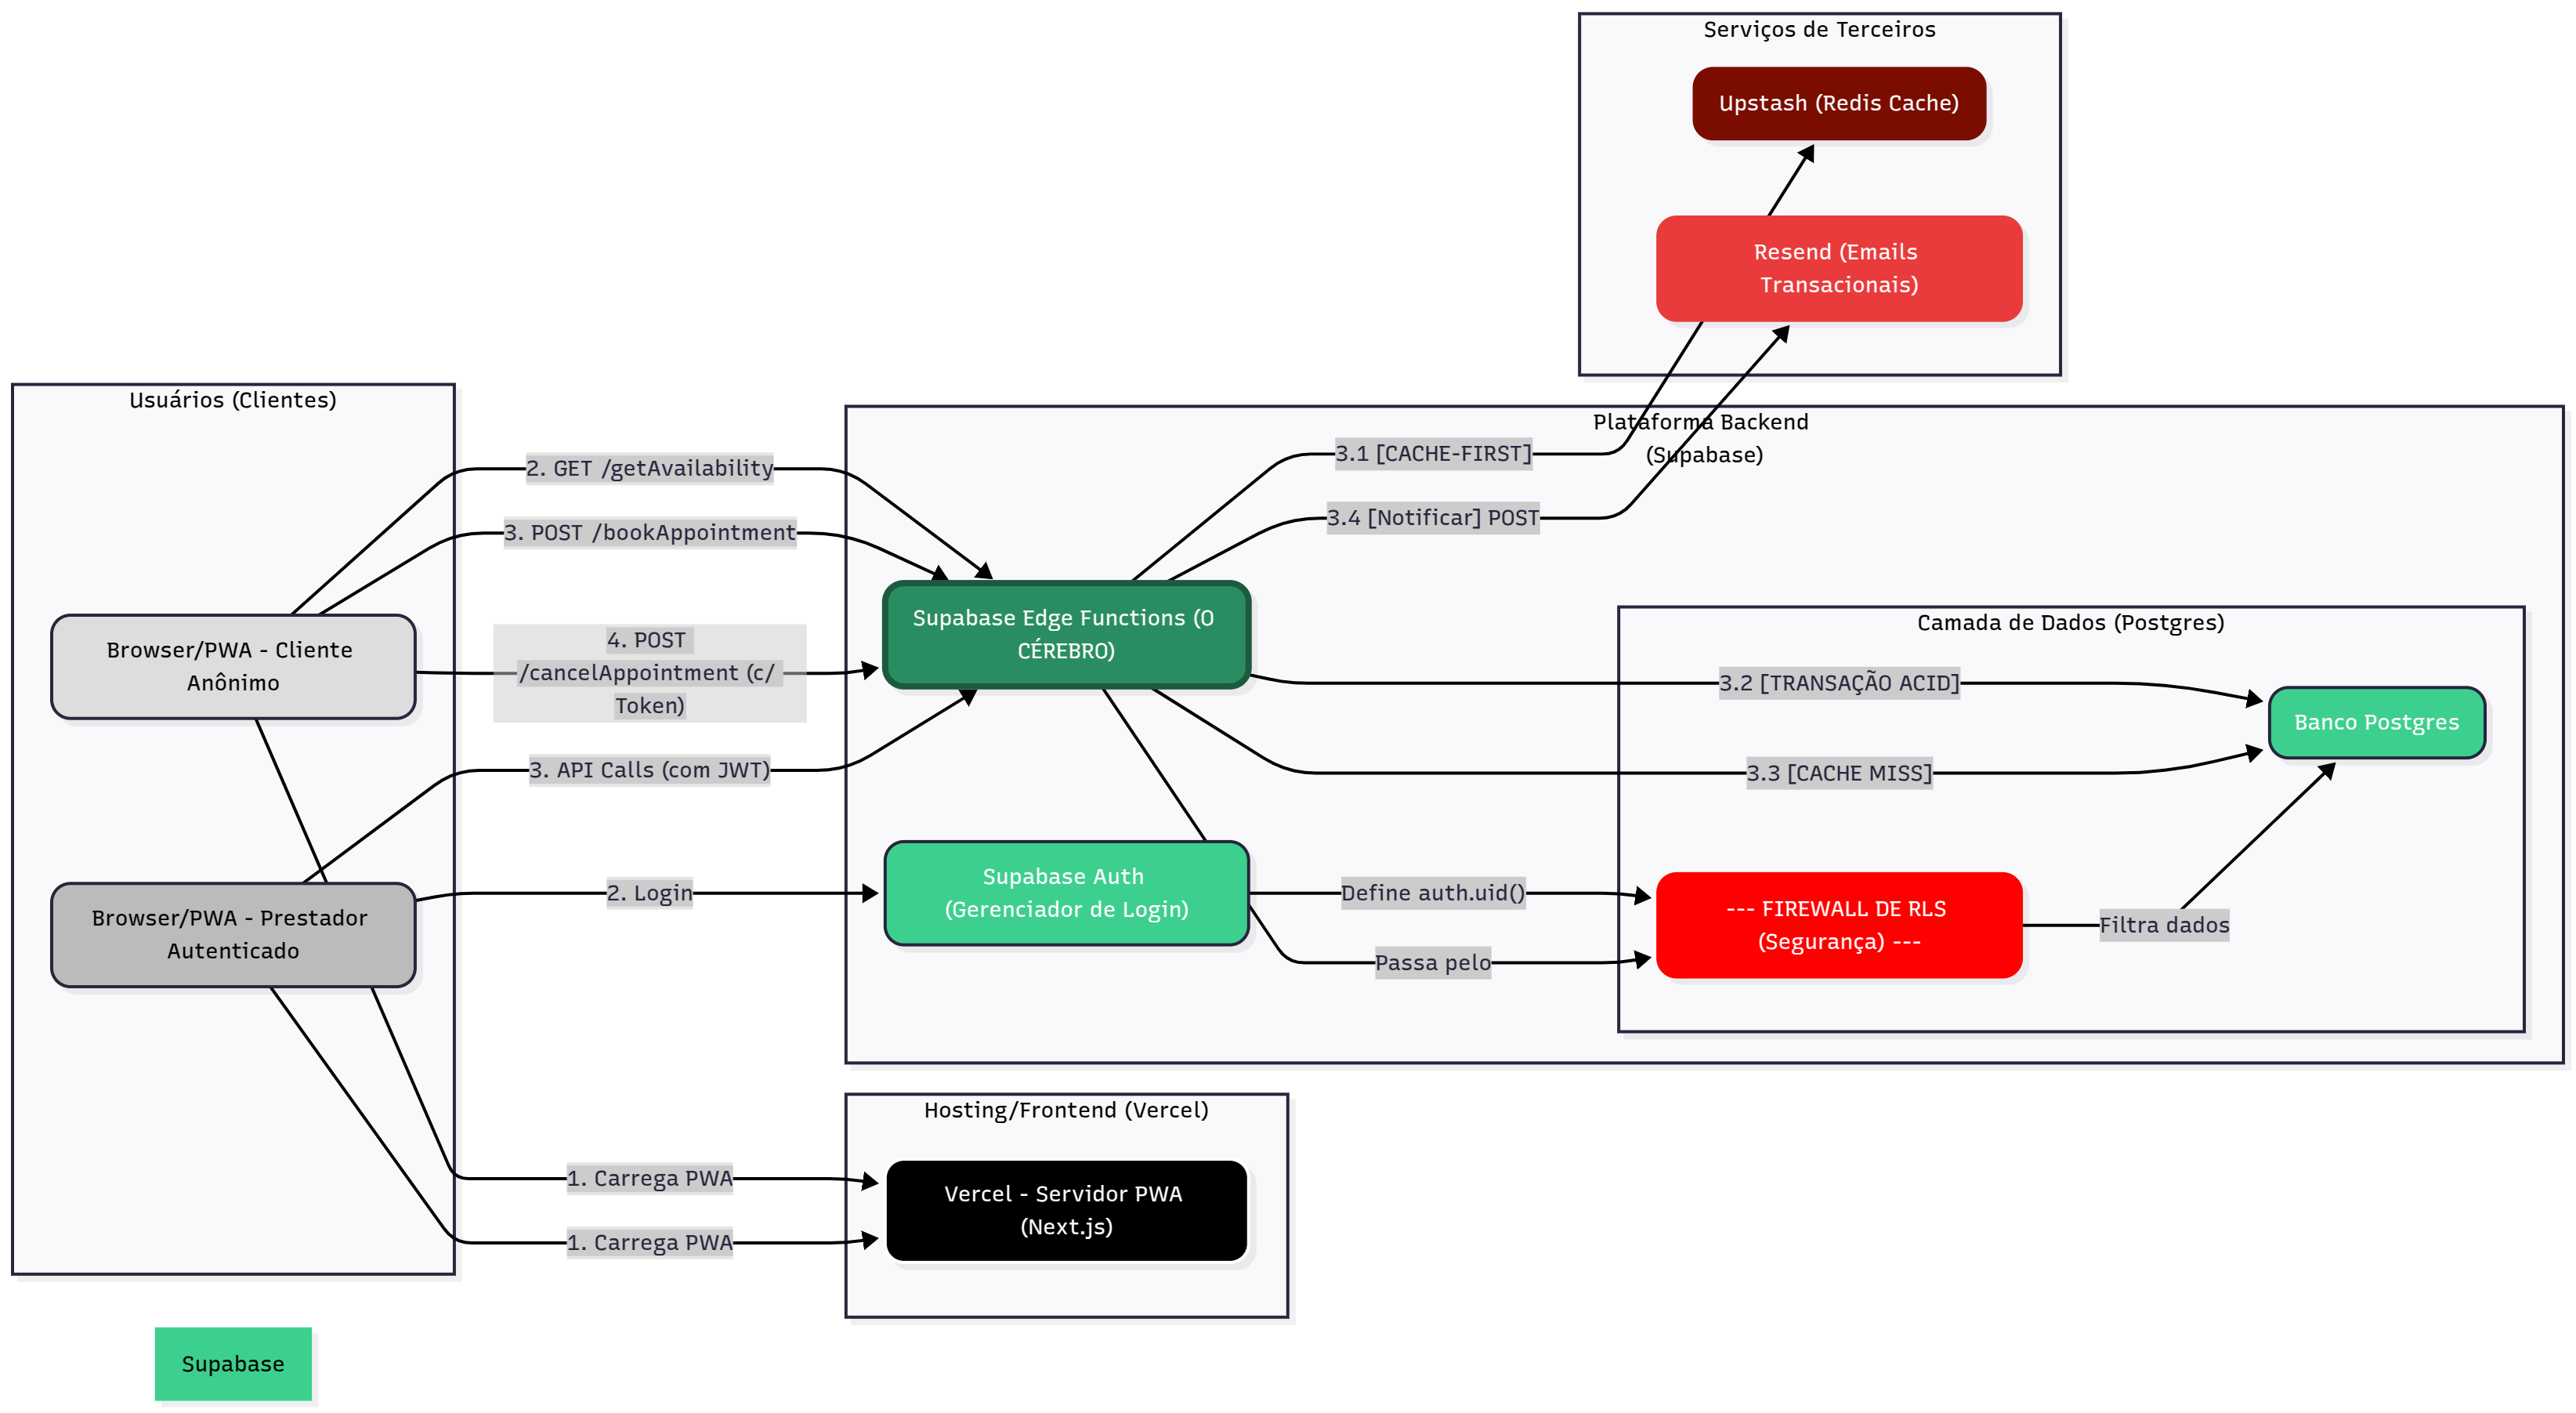
\includegraphics[width=.9\textwidth]{diagrama-arquitetural.png}
\caption{Diagrama Arquitetural e Fluxo de Dados}
\label{arquitetura}
\end{figure}

Os componentes fundamentais da solução são:

\begin{itemize}
    \item \textbf{Frontend:} Aplicação \textit{Progressive Web App} \cite{pwa_optimal_strategies} (PWA) em Next.js, hospedada na Vercel\footnote{https://vercel.com/} e entregue via rede de entrega de conteúdo (do inglês, \textit{Edge Network}).
    \item \textbf{Backend:} O ecossistema Supabase\footnote{https://supabase.com} provê:
        \begin{itemize}
            \item \textbf{Banco de Dados:} PostgreSQL \cite{postgres_isolation} como fonte da verdade (do inglês, \textit{Source of Truth}).
            \item \textbf{Segurança:} Autenticação integrada com segurança em nível de linha (do inglês, \textit{Row Level Security - RLS} \cite{medium_rls_explained}), garantindo isolamento de dados.
            \item \textbf{Orquestração:} Funções \textit{serverless} (Edge Functions) para regras de negócio.
        \end{itemize}
    \item \textbf{Cache:} Redis \cite{redis_invalidation} gerenciado (Upstash\footnote{https://upstash.com/}) para dados voláteis de baixa latência.
    \item \textbf{Mensageria:} Resend\footnote{https://resend.com/} para despacho assíncrono de notificações transacionais (Serviço de email para o envio de confirmações e cancelamentos.).
\end{itemize}

\subsection{Padrão de Leitura: Cache-Aside}
Para mitigar a latência, implementa-se o padrão \textbf{\textit{Cache-Aside}} \cite{medium_caching_essentials}. A aplicação orquestra a busca conforme o algoritmo:

\begin{enumerate}
    \item \textbf{Requisição:} O cliente solicita a disponibilidade via API.
    \item \textbf{Verificação (Look-Aside):} Consulta-se primeiramente o Redis.
    \item \textbf{Cenário \textit{Cache Hit}:} Se o dado existe, retorna-se o JSON, poupando o banco de dados.
    \item \textbf{Cenário \textit{Cache Miss}:} Se ausente, a função consulta o PostgreSQL (realizando os JOINs necessários), serializa o resultado, grava no Redis com tempo de vida (TTL) definido e retorna ao cliente.
\end{enumerate}

Esta abordagem garante consistência eventual (do inglês, \textit{eventually consistent}) com alta performance, penalizando apenas a primeira requisição do período.

\subsection{Padrão de Escrita: Transacional com Invalidação}
A integridade dos dados exige o padrão \textbf{\textit{Write-Invalidate}} dentro de um contexto transacional ACID (atomicidade, consistência, isolamento e durabilidade):

\begin{enumerate}
    \item \textbf{Transação:} A Edge Function inicia uma transação no PostgreSQL.
    \item \textbf{Validação:} Verifica-se a disponibilidade em tempo real (bloqueio de leitura) e insere-se o agendamento.
    \item \textbf{Commit/Rollback:} Em caso de conflito, executa-se o \textit{Rollback} (erro 409). Em sucesso, o \textit{Commit}.
    \item \textbf{Invalidação (Pós-Commit):} Após a persistência, envia-se comando de deleção (\texttt{DEL}) ao Redis para a chave afetada, forçando a atualização do cache na próxima leitura.
    \item \textbf{Notificação:} Dispara-se o email de confirmação assincronamente.
\end{enumerate}

%====================================================================

\section{Requisitos do Sistema}
\justifying
A arquitetura proposta foi definida para satisfazer um conjunto de requisitos funcionais e não-funcionais que garantem a viabilidade e o sucesso do produto.

\subsection{Requisitos Funcionais (RF)}
Os requisitos funcionais definem as operações que os atores (Prestador e Cliente) podem realizar.

\subsubsection{Prestador de Serviço}
\begin{itemize}
    \item \textbf{RF-P01 (Autenticação):} O sistema deve permitir que o Prestador se autentique via Supabase Auth.
    \item \textbf{RF-P02 (Gestão de Perfil):} O Prestador deve poder gerenciar seu perfil e seu \texttt{public\_slug} (URL pública).
    \item \textbf{RF-P03 (Gestão de Grupos de Disponibilidade):} O Prestador deve poder criar, nomear e ativar/desativar grupos de horários (ex: "Horário Comercial").
    \item \textbf{RF-P04 (Gestão de Regras):} O Prestador deve poder definir intervalos de tempo (início/fim) para dias da semana dentro de um grupo.
    \item \textbf{RF-P05 (Gestão de Exceções):} O Prestador deve poder bloquear horários específicos em um dia (ex: "médico às 15h").
    \item \textbf{RF-P06 (Cancelamento de Agendamento):} O Prestador deve poder cancelar um agendamento existente, o que deve disparar uma notificação (via Resend) ao cliente.
\end{itemize}

\subsubsection{Cliente Final}
\begin{itemize}
    \item \textbf{RF-C01 (Consulta de Disponibilidade):} O Cliente anônimo deve poder visualizar os horários disponíveis na URL pública do prestador.
    \item \textbf{RF-C02 (Realização de Agendamento):} O Cliente deve poder agendar um horário sem necessidade de login, fornecendo apenas nome, email e telefone.
    \item \textbf{RF-C03 (Confirmação por Email):} Ao agendar, o Cliente deve receber um email de confirmação contendo um link único de cancelamento (\texttt{cancellation\_token}).
    \item \textbf{RF-C04 (Cancelamento Próprio):} O Cliente deve poder cancelar seu agendamento através do link único, sem intervenção humana.
\end{itemize}

\subsection{Requisitos Não-Funcionais (RNF)}
Os RNF definem os atributos de qualidade da arquitetura.

\begin{itemize}
    \item \textbf{RNF-D01 (Desempenho - Cache-First):} 95\% das requisições de disponibilidade (RF-C01) devem ser respondidas em menos de 100ms (servidas pelo cache).
    \item \textbf{RNF-S01 (Segurança - RLS):} A arquitetura deve implementar Row Level Security. Um prestador autenticado só pode ler/escrever dados que possuam seu \texttt{provider\_id}.
    \item \textbf{RNF-S02 (Segurança - Token):} O cancelamento do cliente (RF-C04) não deve ser possível sem o \texttt{cancellation\_token} único.
    \item \textbf{RNF-C01 (Confiabilidade - ACID):} O agendamento (RF-C02) deve ser uma Transação ACID para garantir integridade e evitar \textit{race conditions}.
    \item \textbf{RNF-U01 (Usabilidade - PWA):} A aplicação deve ser um PWA instalável e com design \textit{Mobile-First}.
    \item \textbf{RNF-U02 (Usabilidade - Fluxo do Cliente):} O fluxo de agendamento do cliente (RF-C01 a C03) deve ser completado em no máximo 3 etapas, sem nenhuma exigência de login ou criação de senha.
\end{itemize}


%=============================================

\section{Protótipo e Implementação da Interface}
\justifying

A validação da arquitetura proposta materializa-se através de um protótipo desenvolvido com foco na usabilidade móvel (\textit{Mobile-First}) e na performance de carregamento. As interfaces foram projetadas para minimizar a fricção cognitiva, permitindo que tanto o prestador quanto o cliente realizem suas tarefas críticas com o mínimo de interações. Mais detalhes sobre a ferramenta estão disponíveis no repositório \footnote{https://github.com/ibaG20/repositorio-tcc}.

\subsection{Visão do Prestador de Serviço}
A área administrativa permite ao microempreendedor gerenciar sua disponibilidade de forma granular, abstraindo a complexidade das regras de negócio em uma interface intuitiva.

As Figuras \ref{fig:config_regras_home} e \ref{fig:config_regras_detalhes} apresenta a tela de configuração de Grupos de Horários, onde o prestador define seus intervalos de trabalho padrão, conforme os requisitos RF-P03 e RF-P04.

\subsection{Jornada do Cliente Final}
A interface pública foca na conversão e na velocidade. Ao acessar o link único do prestador, o cliente visualiza a disponibilidade real (servida via cache Redis) e conclui o agendamento em três etapas, sem necessidade de login.

A Figura \ref{fig:agendamento} ilustra a tela de seleção de horários e o modal de confirmação simplificado.

\begin{figure}[hbt]
    \centering
    % --- PRIMEIRA IMAGEM (ESQUERDA) ---
    \begin{minipage}{0.22\textwidth}
        \centering
        
\includegraphics[width=1\linewidth]{Horários - Home.png} 
        \caption{Grupo de horários}
        \label{fig:config_regras_home}
    \end{minipage}
    % --- SEGUNDA IMAGEM (MEIO) ---
    \begin{minipage}{0.22\textwidth}
        \centering
        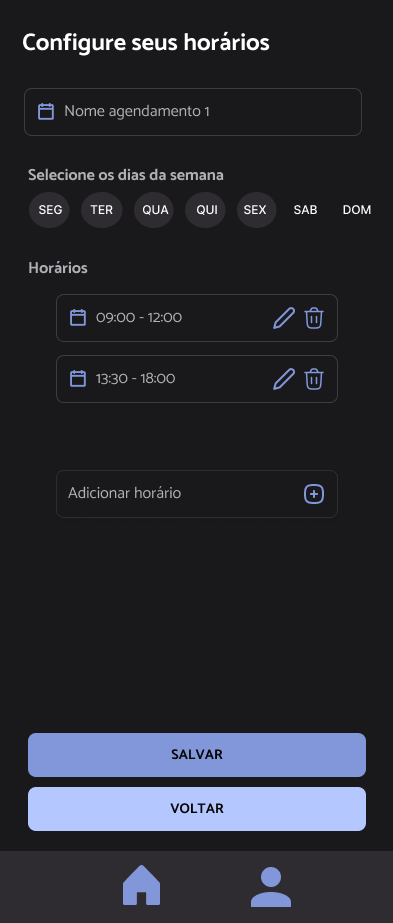
\includegraphics[width=1\linewidth]{Horários - Detalhes.png}
        \caption{Criação de um novo horário }
        \label{fig:config_regras_detalhes}
    \end{minipage}
    % --- TERCEIRA IMAGEM (DIREITO) ---
    \begin{minipage}{0.22\textwidth}
        \centering
        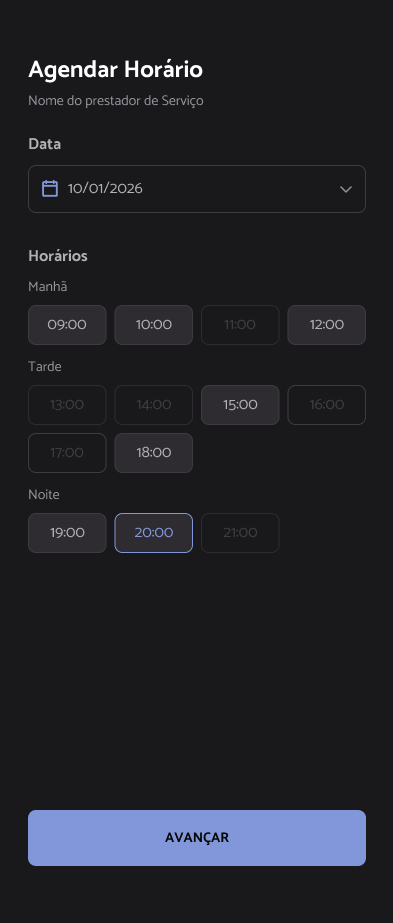
\includegraphics[width=1\linewidth]{Agendamento cliente - Etapa 1.png}
        \caption{Agendar horário}
        \label{fig:agendamento}
    \end{minipage}
    
\end{figure}

%====================================================================

%\clearpage 
\section{Cronograma}

A Tabela \ref{tab:cronograma_detalhado} apresenta o desdobramento operacional das atividades previstas para o semestre letivo, detalhando os entregáveis de cada etapa.

\begin{table}[hbt]
\centering
\caption{Cronograma Detalhado de Desenvolvimento e Escrita}
\label{tab:cronograma_detalhado}
\footnotesize 
\renewcommand{\arraystretch}{1.2} 

\begin{tabularx}{\textwidth}{|c|X|}
\hline
\textbf{Mês} & \textbf{Atividades e Entregáveis} \\ \hline

\textbf{Fev/26} 
& \textbf{Infraestrutura \& Banco de Dados:} Setup do Git/Vercel (CI/CD) $\bullet$ Configuração Supabase (Auth + DB) $\bullet$ Modelagem do Schema (\textit{profiles, rules, appointments}) $\bullet$ Implementação crítica de RLS (\textit{Row Level Security}) $\bullet$ Revisão bibliográfica. \\ \hline

\textbf{Mar/26} 
& \textbf{Backend Serverless \& Cache:} Edge Function de Leitura (Upstash/Redis + \textit{Cache-Aside}) $\bullet$ Edge Function de Escrita (Transação ACID + \textit{bookAppointment}) $\bullet$ Estratégia \textit{Write-Invalidate} $\bullet$ Escrita: Metodologia e Arquitetura. \\ \hline

\textbf{Abr/26} 
& \textbf{Frontend PWA \& Integração:} Interface do Prestador (Regras/Exceções) $\bullet$ Interface Pública do Cliente (\textit{Mobile-First}) $\bullet$ Integração API de Emails (Resend) $\bullet$ Config. PWA (\textit{Manifest/Service Workers}) $\bullet$ Escrita: Desenvolvimento. \\ \hline

\textbf{Mai/26} 
& \textbf{QA, Otimização \& Escrita Final:} Testes de Concorrência (ACID) $\bullet$ Auditoria Lighthouse (Score 90+) $\bullet$ Coleta de métricas (custo/performance) $\bullet$ Escrita: Resultados e Conclusão $\bullet$ \textbf{Depósito da Versão Prévia}. \\ \hline

\textbf{Jun/26} 
& \textbf{Ajustes Finais \& Preparação:} Correção de \textit{bugs} residuais $\bullet$ Refinamento visual (UI/UX) $\bullet$ Elaboração dos slides e roteiro de demo $\bullet$ \textbf{Entrega da Versão Final}. \\ \hline

\textbf{Jul/26} & \textbf{\textsc{Defesa do Trabalho de Conclusão de Curso.}} \\ \hline

\end{tabularx}
\end{table}
%====================================================================

\section{Conclusão}
\justifying

Este trabalho apresentou uma arquitetura de sistema para um PWA de agendamento, removendo a complexidade da abordagem \textit{Offline-First} em favor de uma arquitetura \textit{Cache-First} mais eficiente, barata e performática.

A solução proposta (Supabase, Upstash, Resend) soluciona diretamente os problemas do MEI:
\begin{enumerate}
    \item \textbf{Custo:} A arquitetura \textit{serverless} possui um custo operacional marginal (estimado em R\$ 0,07/usuário/mês), permitindo um modelo de negócio sustentável e acessível.
    \item \textbf{Performance em Redes Ruins:} O uso de cache na borda (Redis) garante que a aplicação seja extremamente rápida e consuma o mínimo de dados móveis, resolvendo na prática o problema da "conectividade precária".
    \item \textbf{Profissionalização:} A automação da jornada do cliente (confirmação e cancelamento por email) eleva o nível de serviço do MEI e elimina a carga operacional do WhatsApp.
\end{enumerate}

A implementação desta arquitetura prova ser uma solução tecnicamente robusta, economicamente viável e socialmente relevante, entregando valor real a milhões de microempreendedores brasileiros.

% ===================================================================
% REFERÊNCIAS BIBLIOGRÁFICAS
% ===================================================================

\begin{thebibliography}{99}

\bibitem{ibge_noticias}
AGÊNCIA IBGE NOTÍCIAS. \textit{Em 2022, Brasil tinha 14,6 milhões de microempreendedores individuais}. Disponível em: \url{https://agenciadenoticias.ibge.gov.br/agencia-noticias/2012-agencia-de-noticias/noticias/41046-em-2022-brasil-tinha-14-6-milhoes-de-microempreendedores-individuais}. Acesso em: 25 ago. 2025.

\bibitem{gov_mapa_empresas}
BRASIL. Ministério do Empreendedorismo, da Microempresa e da Empresa de Pequeno Porte. \textit{Boletim do 1º quadrimestre de 2024 do Mapa de Empresas}. Disponível em: \url{https://www.gov.br/empresas-e-negocios/pt-br/mapa-de-empresas/boletins/mapa-de-empresas-boletim-1o-quadrimestre-2024.pdf}. Acesso em: 30 nov. 2025.

\bibitem{sebrae_digital}
SEBRAE DIGITAL. \textit{A digitalização para pequenos negócios tradicionais}. Disponível em: \url{https://digital.sebraers.com.br/blog/inovacao/digitalizacao-pequenos-negocios-tradicionais/}. Acesso em: 25 ago. 2025.

\bibitem{cetic_tic_domicilios_2024}
CETIC.br. \textit{TIC Domicílios 2024 - Livro Eletrônico}. Disponível em: \url{https://cetic.br/media/docs/publicacoes/2/20250512120132/tic_domicilios_2024_livro_eletronico.pdf}. Acesso em: 30 nov. 2025.

\bibitem{sebrae_pr}
SEBRAE/PR. \textit{Pesquisa Maturidade Digital Dos Pequenos Negócios No Brasil - 2024}. Disponível em: \url{https://sebraepr.com.br/impulsiona/maturidade-digital-dos-pequenos-negocios-no-brasil-2024/}. Acesso em: 25 ago. 2025.

\bibitem{pwa_optimal_strategies}
IJRES. \textit{Progressive Web App}. Disponível em: \url{https://www.ijres.org/papers/Volume-12/Issue-3/1203174180.pdf}. Acesso em: 30 nov. 2025.

\bibitem{postgres_isolation}
POSTGRESQL. \textit{Documentation 18: 13.2. Transaction Isolation}. Disponível em: \url{https://www.postgresql.org/docs/current/transaction-iso.html}. Acesso em: 30 nov. 2025.

\bibitem{medium_rls_explained}
SUPABESE ROW LEVEL SECURITY. \textit{Supabase Row Level Security Explained With Real Examples}. Medium. Disponível em: \url{https://medium.com/@jigsz6391/supabase-row-level-security-explained-with-real-examples-6d06ce8d221c}. Acesso em: 30 nov. 2025.

\bibitem{redis_invalidation}
REDIS.IO. \textit{Cache Invalidation}. Disponível em: \url{https://redis.io/glossary/cache-invalidation/}. Acesso em: 30 nov. 2025.

\bibitem{medium_caching_essentials}
ZHBANKOV, Y. \textit{Caching Essentials: Types, Strategies, and Best Practices}. Medium. Disponível em: \url{https://medium.com/@yaroslavzhbankov/caching-essentials-types-strategies-and-best-practices-459493cc47d9}. Acesso em: 30 nov. 2025.

\end{thebibliography}

\end{document}